\chapter{The Divergence Half}\label{chap:divergence}

An orbit of the Collatz map that never reaches $1$ either enters a cycle or
grows without bound.
The previous chapter dealt with cycles: a cycle is an exact multiplicative coincidence, continued fractions\index{continued fraction} of $\lt$ control how long it would have to be, and Diophantine\index{Diophantine approximation} information alone cannot exclude it (\cref{prop:ch8:insufficient}).
This chapter deals with the other possibility. A divergent orbit is not a
coincidence at all. It is an orbit along which the halvings are, on average,
too few, and the question of whether one exists is a question about averages
along a single deterministic sequence.

The stochastic model of \cref{chap:stochastic} answers that question for an
idealized random orbit, and the answer is no: a random walk with drift\index{drift}
$\log(3/4)$ per stride does not escape. The difficulty, which has been met in
every chapter so far, is that the model describes ensembles of starting values
and the conjecture concerns each starting value separately. In this chapter
we make the gap as precise as we can. We prove a Ces\`aro identity that turns the
divergence half into a statement about the running mean of the halving
exponents (\cref{prop:cesaro}); we show that the obvious empirical test of
that statement carries no information at all; we formulate the statement that
would be needed (\cref{conj:cesaro}) and relate its threshold $\lt$ to the
momentum\index{momentum} coefficient of \cref{chap:smm}; we study the residues of Syracuse
orbits modulo powers of $3$, where the model chain, in which the halving
exponents are independent draws, can be computed
exactly (\cref{lem:ch9:mixing}); and we describe Tao\index{Tao, T.}'s theorem, which is the
deepest result in this direction, and the reason it stops short of every
integer. The chapter ends with three routes to the divergence half and the
points at which they fail.

Throughout, $x_0$ is an odd positive integer, $y_j=S^{(j)}(x_0)$ are the
successive odd iterates under the Syracuse map\index{Syracuse map}, and
\[
  k_j=\vt(3y_{j-1}+1),\qquad\bar k_N=\frac1N\sum_{j=1}^Nk_j ,
\]
so that $y_j=(3y_{j-1}+1)/2^{k_j}$.

\section{Divergent orbits and what is known}\label{sec:ch9:known}

Call the orbit of $x_0$ \emph{divergent} if $\sup_jy_j=\infty$. No divergent
orbit is known, and very little is known about what one would look like. We
collect the elementary facts.

\begin{lemma}[Divergent orbits tend to infinity]\label{lem:ch9:infinity}
If the orbit of $x_0$ is divergent, then $y_j\to\infty$, the values $y_j$ are
pairwise distinct, and no $y_j$ is an integer known to reach $1$; in
particular $y_j>2^{71}$ for all $j$.
\end{lemma}

\begin{proof}
If $y_i=y_j$ for some $i<j$, the orbit is periodic from $i$ on and hence
bounded, so the values are distinct. A sequence of distinct positive integers
takes each value at most once, so for every $B$ only finitely many $y_j$ are at
most $B$, and $y_j\to\infty$. If some $y_j$ reached $1$ the orbit would be
bounded. Every integer below $2^{71}$ reaches $1$ by the computation of
Ba\v{r}ina\index{Barina, D.@Ba\v{r}ina, D.}~\cite{barina2025}, so no $y_j$ lies below $2^{71}$, and $y_j\neq2^{71}$ since $y_j$ is odd.
\end{proof}

Beyond this, the known results about divergence are of two kinds. Density
theorems say that the set of starting values with badly behaved orbits is
small: Terras\index{Terras, R.}~\cite{terras1976,terras1979} and, independently,
Everett\index{Everett, C. J.}~\cite{everett1977} (\cref{thm:density}) show that almost every integer, in natural
density, falls below its starting value; Korec\index{Korec, I.}~\cite{korec1994} shows that
almost every orbit falls below $n^{\gamma}$ for each $\gamma>\log3/\log4$; and
Tao\index{Tao, T.}~\cite[Theorem~1.3]{tao2022} shows that, for every function $f$ tending to
infinity, almost every orbit, in logarithmic density, falls below $f(n)$. None of these statements implies that
the set of starting values with divergent orbits has density zero, let alone
that it is empty, because an orbit that falls below its starting value may rise
again, and its later values are not uniformly distributed in any residue
class. Counting theorems, of which the strongest is due to Krasikov\index{Krasikov, I.} and
Lagarias\index{Lagarias, J. C.}~\cite{krasikov2003}, give lower bounds for the number of integers that
provably reach $1$; we return to them in \cref{sec:ch9:krasikov}.

The second kind of result is structural: a divergent orbit, if one exists,
must be atypical in a precise statistical sense. The rest of this section and
the next make that precise.

\begin{remark}[The $2$ adic picture]\label{rem:ch9:adic}
By \cref{thm:ch2:conj}, the accelerated map\index{accelerated map} on the $2$ adic integers is
conjugate to the shift on parity sequences, and Haar measure\index{Haar measure} corresponds to
fair coin flips (\cref{prop:ch2:haar}). By the strong law of large numbers,
Haar almost every $2$ adic integer has a $T$ orbit in which the frequency of
odd steps is $\tfrac12$. We shall see in \cref{cor:ch9:freq} that a divergent
orbit must have a frequency of odd steps of at least $1/\lt\approx0.631$ in the
limit. The set of $2$ adic integers with this property has Haar measure zero.
This is no contradiction, since the positive integers are themselves a set of
Haar measure zero, but it is a measure of how atypical a divergent orbit must
be. Counting parity words gives a quantitative version: among the $2^n$ words
of length $n$, the number with at least $qn$ ones, $q=1/\lt$, is
$2^{nH(q)+o(n)}$, where $H(q)=-q\log_2q-(1-q)\log_2(1-q)\approx0.9500$. The
fraction of residue classes modulo $2^n$ whose first $n$ steps of $T$ contain
at least $n/\lt$ odd steps therefore decays like $2^{-0.05n}$, the rate $e^{-D}\approx
0.9659$ per step of \cref{thm:density} and \cref{sec:ch3:lyapunov}.
\end{remark}

\section{The Ces\`aro identity}\label{sec:ch9:cesaro}

The following identity is the telescoped form of the stride formula
\eqref{eq:ch2:stride}. It is elementary, and its value lies entirely in what it
does and does not say.

\begin{proposition}[Ces\`aro identity]\label{prop:cesaro}
For every odd $x_0$ and every $N\geq1$,
\begin{equation}\label{eq:ch9:cesaro}
  \log y_N-\log x_0=\sum_{j=1}^{N}\log\Bigl(3+\frac{1}{y_{j-1}}\Bigr)
  -N\bar k_N\log2 .
\end{equation}
Equivalently,
\begin{equation}\label{eq:ch9:kbar}
  \bar k_N=\lt+\frac{1}{N}\Bigl(\log_2x_0-\log_2y_N+\sum_{j=1}^{N}
  \log_2\Bigl(1+\frac{1}{3y_{j-1}}\Bigr)\Bigr).
\end{equation}
Consequently, if the orbit of $x_0>1$ reaches $1$ at stride $N$, then
\begin{equation}\label{eq:ch9:forced}
  \bar k_N\;>\;\lt+\frac{\log_2x_0}{N}\;>\;\lt .
\end{equation}
\end{proposition}

\begin{proof}
Taking logarithms in $2^{k_j}y_j=3y_{j-1}+1$ gives
$\log y_j-\log y_{j-1}=\log(3+1/y_{j-1})-k_j\log2$, and summing over
$j=1,\ldots,N$ gives \eqref{eq:ch9:cesaro}. Writing
$\log(3+1/y)=\log3+\log(1+1/(3y))$, dividing by $N\log2$ and rearranging
gives \eqref{eq:ch9:kbar}. If $y_N=1$ then $\log_2y_N=0$ and every correction
term $\log_2(1+1/(3y_{j-1}))$ is positive, which gives \eqref{eq:ch9:forced}.
\end{proof}

The identity converts the conjecture into a statement about the running mean
of the halving exponents. Its consequence for divergent orbits is the
following.

\begin{corollary}[The running mean along a divergent orbit]\label{cor:ch9:freq}
If the orbit of $x_0$ is divergent, then
\[
  \limsup_{N\to\infty}\bar k_N\;\le\;\lt .
\]
Equivalently, the fraction of odd steps among the first $n$ steps of the
accelerated map\index{accelerated map} satisfies $\liminf_n(\text{fraction})\geq1/\lt\approx0.6309$,
and among the first $n$ steps of the standard map\index{standard map}
$\liminf_n(\text{fraction})\geq1/(1+\lt)\approx0.3869$.
\end{corollary}

\begin{proof}
By \cref{lem:ch9:infinity}, $y_j\to\infty$, so the correction terms
$\log_2(1+1/(3y_{j-1}))$ tend to zero and so does their Ces\`aro mean; and
$\log_2y_N>0$ for all large $N$. Inserting both facts in \eqref{eq:ch9:kbar}
gives $\bar k_N\le\lt+o(1)$. The first $N$ strides contain $N$ odd steps and
$N\bar k_N$ steps of $T$, or $N(1+\bar k_N)$ steps of $T_0$. If step $n$ of
$T$ falls in stride $N+1$, then at least $N$ of the first $n$ steps are odd and
$n\le(N+1)\bar k_{N+1}\le(N+1)(\lt+o(1))$, so the fraction of odd steps is at
least $N/((N+1)(\lt+o(1)))$, which tends to $1/\lt$. The same count with
$1+\bar k_{N+1}$ in place of $\bar k_{N+1}$ gives the statement for $T_0$.
\end{proof}

The typical values are $\bar k_N\to2$, an odd fraction of $\tfrac12$ for $T$
and $\tfrac13$ for $T_0$ (\cref{prop:ch3:standard}). A divergent orbit must
sustain more than $63$ percent odd steps under $T$, against a typical $50$.

\subsection{A pitfall: the identity is not a test}

Since a divergent orbit must have $\limsup\bar k_N\le\lt$, it is natural to
compute $\bar k_N$ along many orbits and observe that it stays above $\lt$.
The computation is easy and the result is striking.

\begin{remark}[A tempting but uninformative computation]\label{rem:ch9:circular}
For all $2500$ odd starting values $3\le x_0\le5001$ we computed $\bar k_N$ at
the stride $N$ at which the orbit reaches $1$. The minimum is $1.7073$, the
mean is $2.2473$, and every value lies above the threshold $\lt=1.5850$; the
identity \eqref{eq:ch9:cesaro} holds along every orbit with a maximum rounding
residual of about $3\times10^{-14}$. One might present this as evidence
for the divergence half. It is not evidence of any kind. The orbits in the scan
were selected by the property that they reach $1$, and by
\eqref{eq:ch9:forced} every such orbit satisfies $\bar k_N>\lt$ identically.
No outcome of the computation could have been different. The minimum $1.7073$
is $70/41$, attained at $x_0=27$ (\cref{ex:ch2:27}), and it measures the spread
of $\bar k$ over terminating orbits; it says nothing about orbits that do not
terminate.
\end{remark}

The same lesson appears in a sharper form for long orbits. For three odd
starting values chosen at random near $2^{1000}$, $2^{2000}$ and $2^{4000}$, the
orbits reached $1$ after $N=2773$, $4566$ and $9507$ strides, with final means
$\bar k_N=1.94555$, $2.02300$ and $2.00568$. By \eqref{eq:ch9:kbar} with
$y_N=1$, these are
\[
  \bar k_N=\lt+\frac{\log_2x_0}{N}+\frac1N\sum_{j}\log_2\Bigl(1+\frac1{3y_{j-1}}\Bigr),
\]
and the last term is below $10^{-4}$ in all three cases; the values of
$\lt+(\log_2x_0)/N$ are $1.94547$, $2.02293$ and $2.00565$. So the final mean
of the halving exponents carries no information beyond the number of strides,
which is itself a reformulation of the total stopping time\index{stopping time}. What does carry
information is the behaviour of $\bar k_N$ along the way, at strides $N$ when
the orbit is still far from $1$, and that is what \cref{fig:ch9:kbar} shows.

\begin{figure}[t]
\centering
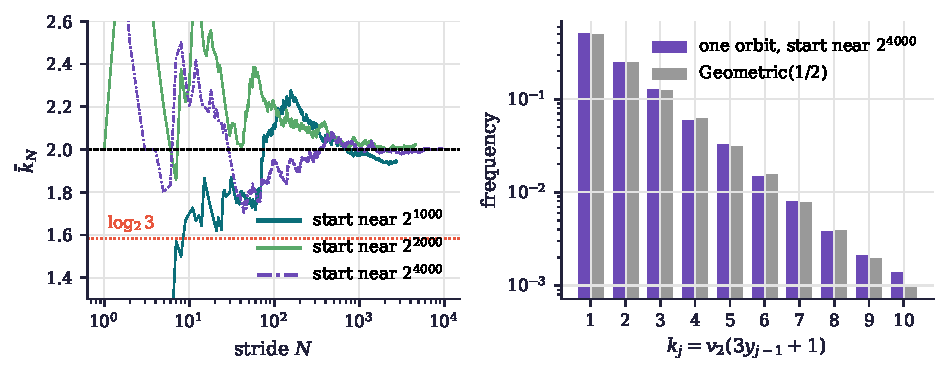
\includegraphics[width=\textwidth]{figures/ch9_kbar.pdf}
\caption{Left: the running mean $\bar k_N$ along three orbits started at random
odd integers near $2^{1000}$, $2^{2000}$ and $2^{4000}$, with the Geometric mean
$2$ (dashed) and the threshold $\lt$ (dotted). Right: the frequencies of the
halving exponents along the orbit from near $2^{4000}$ against the
Geometric$(\tfrac12)$ law, on a logarithmic scale.}
\label{fig:ch9:kbar}
\end{figure}

\section{The Ces\`aro liminf conjecture}\label{sec:ch9:conj}

The divergence half of the conjecture can now be stated in the form the
identity suggests.

\begin{conjecture}[Ces\`aro liminf]\label{conj:cesaro}
For every odd $x_0$,
\[
  \liminf_{N\to\infty}\frac1N\sum_{j=1}^Nk_j\;>\;\lt .
\]
\end{conjecture}

\begin{sloppypar}
Along an orbit that reaches $1$ the exponents are eventually all equal to $2$, since $S(1)=1$ with $k=2$, and along an orbit that enters a cycle with $r$ odd elements and $s$ halvings in one turn their mean tends to $s/r>\lt$ (\cref{lem:cycleid}); so \cref{conj:cesaro} holds for every bounded orbit.
By \cref{cor:ch9:freq}, every divergent orbit has $\liminf\bar k_N\le\limsup\bar k_N\le\lt$, so \cref{conj:cesaro} holds if and only if there is no divergent orbit.
It is therefore exactly equivalent to the divergence half of
the Collatz conjecture\index{Collatz conjecture}, and its interest lies not in being weaker but in
pointing at a mechanism. Under the Geometric law of \cref{prop:geom} the
exponent at a uniformly random odd residue has mean $2$, and if the exponents along an orbit obeyed the strong
law of large numbers we would have $\bar k_N\to2>\lt$, with a margin of
$2-\lt\approx0.415$. The margin belongs to the model: along a divergent orbit there is none, by \cref{cor:ch9:freq}.
A proof of \cref{conj:cesaro} would need much less than a Geometric law for the exponents along unbounded orbits, or full equidistribution\index{equidistribution} of their residues (\cref{sec:ch9:equi}): one needs only that along no orbit $\limsup_N\bar k_N\le\lt$, that is, that the mean of the exponents cannot fall short of $2$ by $2-\lt\approx0.415$ or more in the limit.
\end{sloppypar}

The threshold has a second reading. Write
\[
  \lt=1+\beta,\qquad\beta=\frac{\log(3/2)}{\log2}\approx0.585 ,
\]
where $\beta$ is the Switching MM\index{Switching MM} momentum\index{momentum} coefficient of \cref{chap:smm}. Every
stride contains one forced halving, since $k_j\geq1$, and the conjecture
asks that the \emph{extra} halvings $k_j-1$ exceed $\beta$ on average. In the
optimization reading of the book, the tripling and the forced halving together
form the overshoot $\log(3/2)$, and $\beta$ is that overshoot measured in units
of one halving; the extra halvings are the corrective descent. The Geometric
law gives $\E[k-1]=1$, so the correction exceeds the overshoot by a factor
$1/\beta\approx1.71$. The divergence half asks that this inequality, which
holds in expectation, hold along every orbit in the long run.

\section{Equidistribution of the halving exponent along orbits}\label{sec:ch9:equi}

The right panel of \cref{fig:ch9:kbar} shows the empirical law of $k_j$ along
the single orbit from near $2^{4000}$. Over its $9507$ strides the frequencies
of $k=1,2,3,4,5$ are $0.5026$, $0.2462$, $0.1271$, $0.0596$, $0.0330$, against
$0.5$, $0.25$, $0.125$, $0.0625$, $0.03125$; the sample mean is $2.0057$ and the
sample variance $2.0913$, against $2$ and $2$. The running means in the left
panel settle near $2$ and stay well clear of $\lt$ once the orbit is past its
first few dozen strides.

Part of this agreement is a theorem and part of it is not. Extending
\cref{prop:ch3:exact} to strides: if $x_0$ is uniformly distributed over the odd
residues modulo $2^K$, the parity vector\index{parity vector} of length $K$ is uniform over the words that begin with $1$, so the
halving exponents $k_1,k_2,\ldots$ are independent Geometric$(\tfrac12)$ for
as long as their sum stays below $K$. A starting value near $2^{4000}$ thus
controls roughly the first $2000$ strides, about a fifth of its orbit. After
that the exponents are determined by bits that the orbit has manufactured
itself, through the multiplications by $3$ and the additions of $1$, and no
theorem says they remain Geometric.
The figure says that they do, and so do the other long orbits computed in this book, such as the giant orbit of the gallery (Plate~\ref{fig:gal:giant}); this is the phenomenon that has never been proved.
Note also that the theorem concerns an ensemble of starting values,
whereas the figure shows one orbit. Even over the first $2000$ strides,
\cref{prop:ch3:exact} says only that most residue classes produce Geometric
statistics, not that the particular orbit drawn does.
The same is true of the quantitative form due to Tao\index{Tao, T.}, which shows that the first halving exponents of a starting value drawn at random from a long range are close in total variation to independent Geometric$(\tfrac12)$ draws~\cite[Proposition~1.9]{tao2022}.

What one would like is a statement of the form: for every odd $x_0$ whose orbit is divergent, and every $m$, the residues $y_j\bmod2^m$ are asymptotically equidistributed\index{equidistribution} over the odd classes in the Ces\`aro sense. Since $y_{j-1}\bmod2^m$ determines $\min(k_j,m)$, \cref{prop:geom} would then give $\liminf_N\bar k_N\ge2-2^{1-m}$ for every $m$, so $\liminf_N\bar k_N\ge2$ along such an orbit, against $\limsup_N\bar k_N\le\lt$ from \cref{cor:ch9:freq}; the statement is therefore equivalent to the divergence half, as \cref{conj:cesaro} is. It cannot be asked of every orbit: an orbit that reaches $1$ stays there, so its residues are eventually constant and are not equidistributed for any $m\geq2$. For orbits that reach $1$ the natural statement concerns random starting values, as problem O2 of \cref{chap:open} does for the residues modulo $3^a$.

\section{The $3$ adic side: the model chain modulo $3^a$}\label{sec:ch9:spectral}

The $2$ adic residues of the iterates determine the halving exponents; the
$3$ adic residues are where the multiplication by $3$ leaves its mark, and it
is on the $3$ adic side that Tao\index{Tao, T.} found the leverage for his theorem. Here the
picture is clean enough to compute exactly.

Since $3y+1\equiv1\pmod3$ and $2$ is invertible modulo $3$, every Syracuse
iterate $S(y)$ is prime to $3$. Fix $a\geq1$ and $M=3^a$, and let $U_a$ be the
set of $2\cdot3^{a-1}$ units modulo $M$. For $r\in U_a$ define the matrix
\begin{equation}\label{eq:ch9:P}
  P_a(s,r)=\sum_{k\geq1}2^{-k}\,\mathbb{I}\bigl[(3r+1)2^{-k}\equiv s\pmod M\bigr],
  \qquad r,s\in U_a ,
\end{equation}
in which $\mathbb{I}$ is the indicator function, $2^{-k}$ inside it denotes the inverse of $2^k$ modulo $M$, and the weight $2^{-k}$ in front of it is the real number. Column $r$ of $P_a$
is the law of $S(y)\bmod M$ when $y\equiv r\pmod M$ and the halving exponent is
an independent Geometric$(\tfrac12)$ variable.

\begin{lemma}[The one step matrix is exact]\label{lem:ch9:exact}
For each $r\in U_a$ and $s\in U_a$,
\[
  \lim_{X\to\infty}\frac{\#\{y\le X:\ y\text{ odd},\ y\equiv r,\ S(y)\equiv s\pmod M\}}
  {\#\{y\le X:\ y\text{ odd},\ y\equiv r\pmod M\}}=P_a(s,r).
\]
More generally, for each fixed $J$, as $X\to\infty$ the joint law of
$(y\bmod M,k_1,\ldots,k_J)$ for $y$ uniform over the odd integers up to $X$
converges to the product of the uniform law and $J$ independent
Geometric$(\tfrac12)$ laws.
\end{lemma}

\begin{proof}
Fix exponents $k_1,\ldots,k_J$ with sum $s_J$. By \cref{thm:terras} (in its
Syracuse form, of which \cref{prop:geom} is the one stride case), the odd $y$ with these exponents form a
single residue class modulo $2^{s_J+1}$. By the Chinese remainder theorem its
intersection with a class modulo $3^a$ is a single class modulo
$2^{s_J+1}3^a$, whose density among the odd integers is
$2^{-s_J}\cdot3^{-a}$. This is the product law. Given $k_1=k$ and
$y\equiv r$, the residue of $S(y)=(3y+1)2^{-k}$ modulo $M$ is
$(3r+1)2^{-k}$, which gives the first statement.
\end{proof}

So the one step transition frequencies are not a model: they are exact
limits. A model enters only when the matrix is iterated, since iterating
assumes that the exponent at each stride is independent of the current residue and of the past along the
orbit. We call the Markov chain on $U_a$ with transition matrix $P_a$, in which the halving exponents are independent Geometric$(\tfrac12)$ draws at every stride, the \emph{model chain}.
By the second half of \cref{lem:ch9:exact} its assumption is again
exact for an ensemble of starting values over any fixed number of strides,
and the residues $y_j\bmod M$ for a uniformly random large $y_0$ then form,
in the limit, a Markov chain with transition matrix $P_a$. For a single orbit
nothing of the kind is known: along an orbit the exponents are determined by the iterates, and the Syracuse map does not induce a Markov chain on residues modulo $M$.

\begin{lemma}[Exact mixing in $a$ strides]\label{lem:ch9:mixing}
For $0\le j\le a$, column $r$ of $P_a^{\,j}$ depends on $r$ only through
$r\bmod3^{a-j}$. In particular $P_a^{\,a}=\pi_ae^{\top}$, where $e$ is the vector of ones: all columns of $P_a^{\,a}$ equal
the stationary law $\pi_a$ of $P_a$, so the model chain is exactly stationary after $a$ strides from every starting residue.
Consequently the eigenvalue $1$ of $P_a$ is simple and every other eigenvalue is zero: the characteristic polynomial of $P_a$ is $\lambda^{|U_a|-1}(\lambda-1)$.
\end{lemma}

\begin{proof}
Let $K_1,K_2,\ldots$ be independent Geometric$(\tfrac12)$ and define the random
map $\phi_i(r)=(3r+1)2^{-K_i}\bmod M$. By induction,
\[
  \phi_j\circ\cdots\circ\phi_1(r)\equiv3^j2^{-(K_1+\cdots+K_j)}r+c_j\pmod M,
\]
where $c_j$ depends on $K_1,\ldots,K_j$ only. The first term depends on $r$ only
through $r\bmod3^{a-j}$, and vanishes modulo $M$ for $j=a$. Column $r$ of
$P_a^{\,j}$ is the law of this composition, which proves the first two claims.
The matrix $P_a^{\,a}=\pi_ae^{\top}$ has rank one and trace $e^{\top}\pi_a=1$, so its eigenvalues, counted with multiplicity, are $1$ once and $0$ otherwise.
They are the $a$th powers of the eigenvalues of $P_a$, and $1$ is an eigenvalue of $P_a$ because $e^{\top}P_a=e^{\top}$; hence $1$ is simple and every other eigenvalue of $P_a$ is zero.
\end{proof}

The identity in the proof is Tao\index{Tao, T.}'s~\cite[eq.~(1.21)]{tao2022}: the residue of the $m$th Syracuse iterate modulo $3^a$ depends only on the halving exponents once $m\geq a$. His recursion~\cite[Lemma~1.12]{tao2022} is one step of the model chain, and he notes that the law of his Syracuse random variable is the unique stationary measure of the $3$ adic chain $x\mapsto(3x+1)/2^k$ with $\Prob(k)=2^{-k}$~\cite[Remark~1.13]{tao2022}. What \cref{lem:ch9:mixing} adds is a restatement in the form of a finite Markov chain, $P_a^{\,a}=\pi_ae^{\top}$, from which the spectrum follows. The order matters: the converse inference fails, since a zero spectrum off the eigenvalue $1$ only makes $P_a-\pi_ae^{\top}$ nilpotent, which by itself would allow the chain as many as $|U_a|-1$ strides to become stationary. Nor does the proof use the law of the halving exponents beyond their independence of the current residue; that independence is the model's assumption, and it fails along an actual orbit, where the exponents are determined by the iterates.

The stationary law $\pi_a$ is the law of the \emph{Syracuse random variable}
\[ \sum_{m=1}^{a}3^{m-1}2^{-(K_1+\cdots+K_m)}\bmod3^a \] of Tao~\cite[eq.~(1.22)]{tao2022}, written in the index reversed form of~\cite[Remark~1.13]{tao2022}; the
reversal of the order of the $K_i$ relative to the proof does not change the
law. For $a=1$ it is $(\tfrac13,\tfrac23)$ on the residues $1,2$, since
$S(y)\equiv2^{-k}\equiv2^k\pmod3$ and $k$ is odd with probability $\tfrac23$.
For $a=2$, on the residues $1,2,4,5,7,8$ modulo $9$, it is
\[
  \pi_2=\tfrac1{63}\,(8,\;16,\;11,\;4,\;2,\;22).
\]
These laws are far from uniform, and the distance from uniform does not
shrink with $a$: the total variation distance from $\pi_a$ to the uniform law
on $U_a$ is $0.278$, $0.346$, $0.371$, $0.389$, $0.399$, $0.407$ for
$a=2,\ldots,7$.
For $a=3$ the most likely unit, $26$, is $29$ times as likely as the least likely, $25$; only $5$ of the $18$ units have probability within a factor $\tfrac32$ of $\tfrac1{18}$, and the median probability is $0.038$, against the mean $\tfrac1{18}\approx0.056$. Tao states that his Syracuse random variables are not uniformly distributed (\cite[Remark~1.15]{tao2022} and the paragraph before his Proposition~1.14); what he proves is approximate uniformity at fine $3$ adic scales (\cref{sec:ch9:tao}).

\begin{figure}[t]
\centering
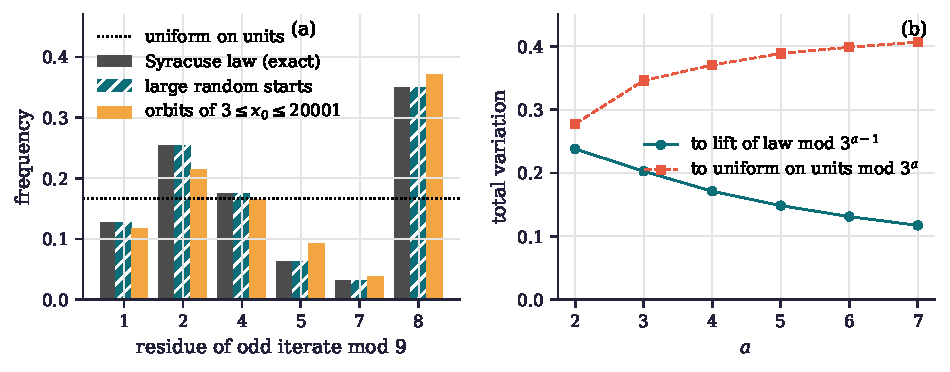
\includegraphics[width=\textwidth]{figures/ch9_syrlaw.pdf}
\caption{Left: frequencies of the residues modulo $9$ of odd Syracuse iterates, against the exact Syracuse law $\pi_2$ and the uniform law on units (dotted). In each group of three bars, the left bar is $\pi_2$, the middle bar $3000$ random starting values near $2^{511}$, strides $3$ to $102$, and the right bar all odd iterates of the orbits of $3\le x_0\le20001$, pooled over orbits that share their tails. Right: total variation distance from $\pi_a$ to the lift of $\pi_{a-1}$ (circles) and to the uniform law on units modulo $3^a$ (squares).}
\label{fig:ch9:syrlaw}
\end{figure}

\Cref{fig:ch9:syrlaw} compares $\pi_2$ with residue frequencies along actual
orbits. For $3000$ random starting values near $2^{511}$, using strides $3$ to
$102$, the empirical law is within total variation $0.0009$ of $\pi_2$; this is
a regime in which \cref{lem:ch9:exact} applies, and the agreement is a theorem
up to sampling error. For the orbits of the small odd starting values
$3\le x_0\le20001$, run to $1$, the distance is $0.058$; but these orbits share
their tails, so their pooled counts are not samples from the model law: their
roughly $317\,000$ odd iterates take only about $12\,000$ distinct values, and
$94$ percent of the orbits end with the same final stride, from $5$ through $16$ to $1$.

\begin{remark}[A pitfall: the wrong null hypothesis]\label{rem:ch9:null}
It is natural to test the $3$ adic equidistribution\index{equidistribution} of Collatz orbits by
comparing residue frequencies modulo $9$ with the uniform law on the six units,
or worse on all nine residues, with a chi squared test.
Such a test rejects decisively for every long orbit in this chapter, and the rejection means nothing.
Residues divisible by $3$ never occur after the first stride, and the correct
null hypothesis on the units is the Syracuse law $\pi_2$, which puts weight
$22/63\approx0.35$ on the residue $8$ and $2/63\approx0.03$ on the residue $7$.
Equidistribution in the sense that matters for Tao's theorem is
equidistribution with respect to the Syracuse law, not with respect to Haar
measure on the units.
\end{remark}

\subsection{A pitfall: odd representatives modulo $27$}

Since every Syracuse iterate is odd, one might build the chain modulo $27$ on the nine odd representatives
\[
  1,\ 5,\ 7,\ 11,\ 13,\ 17,\ 19,\ 23,\ 25
\]
of the units in $[1,27)$, recording a transition $r\to s$ whenever an odd $y\equiv r$ has
$S(y)\equiv s\pmod{27}$ with both $r$ and $s$ in this set. The resulting matrix appears to have a respectable spectral gap, and it is worth seeing why the gap means nothing.

\begin{remark}[A spurious spectral gap]\label{rem:ch9:oddreps}
Let $\hat P$ be the empirical transition matrix of the nine state chain just described, estimated from all odd $y\le10^6$ not divisible by $3$, with each column normalized to sum to one. Its eigenvalue of second largest modulus has modulus $0.5198$, and the limiting matrix, obtained by restricting $P_3$ of \eqref{eq:ch9:P} to the nine states and renormalizing its columns, has a complex conjugate pair of eigenvalues of modulus $0.5202$; taken at face value, this is a spectral gap\index{spectral gap} of about $0.48$. It is not the mixing rate of the model chain, nor of anything else attached to the dynamics. Since $27$ is odd, every residue class modulo $27$ contains integers of both parities, so whether the representative of $y$ in $[0,27)$ is odd says nothing about $y$, and the set of odd $y$ with odd representatives is not invariant under $S$: $55\equiv1\pmod{27}$, while $S(55)=83\equiv2\pmod{27}$. The restricted matrix conditions, at every stride, on a set that the dynamics leaves, and its eigenvalues are artefacts of the conditioning. The model chain is $P_3$ on all eighteen units, which by \cref{lem:ch9:mixing} is exactly stationary\index{mixing} after three strides, so that its eigenvalues other than $1$ are all zero.
\end{remark}

The empirical and limiting values agree, as they must, since by \cref{lem:ch9:exact} the empirical matrix converges to the restricted limiting matrix; the agreement shows only that the restricted matrix has been computed correctly. \Cref{tab:ch9:moduli} compares the restricted matrices with the model chains for the moduli $9$, $27$, $81$ and $243$.

\begin{table}[t]
\centering
\caption{Transition matrices on residues modulo $3^a$. Left block: the matrix restricted
to odd representatives, second eigenvalue modulus from the empirical matrix
(odd $y\le10^6$) and from the limiting matrix. Right block: the model chain on
all units; rank of $P_a^{\,j}$ for $j=a-1,a$, and the largest total variation
distance between a column of the empirical matrix and the corresponding column
of $P_a$.}
\label{tab:ch9:moduli}
\begin{tabular}{@{}rrccrcc@{}}
\toprule
& \multicolumn{3}{c}{Odd representatives} & \multicolumn{3}{c}{All units}\\
\cmidrule(lr){2-4}\cmidrule(l){5-7}
$3^a$ & States & Empirical & Limit & States & Ranks & Column TV\\
\midrule
$9$ & $3$ & $0.0000$ & $0.0000$ & $6$ & $2,\ 1$ & $<10^{-4}$\\
$27$ & $9$ & $0.5198$ & $0.5202$ & $18$ & $2,\ 1$ & $0.0002$\\
$81$ & $27$ & $0.7593$ & $0.7596$ & $54$ & $2,\ 1$ & $0.0006$\\
$243$ & $81$ & $0.7462$ & $0.7461$ & $162$ & $2,\ 1$ & $0.0014$\\
\bottomrule
\end{tabular}
\end{table}

The table was computed as follows. For each modulus we formed the counts of
pairs $(y\bmod3^a,S(y)\bmod3^a)$ over odd $y\le10^6$ not divisible by $3$,
normalized each column to sum to one, and computed eigenvalues with a standard
dense solver; the limiting matrices are given by \eqref{eq:ch9:P} with the sum
over $k$ folded modulo the order $2\cdot3^{a-1}$ of $2$ modulo $3^a$; ranks were
computed with tolerance $10^{-9}$. The restricted matrices have second
eigenvalues that do not decrease with the modulus and bear no relation to the
mixing of the model chain, which is exactly stationary after $a$ strides, as
\cref{lem:ch9:mixing} predicts, while the empirical one step matrices are close
to the limiting ones, as \cref{lem:ch9:exact} predicts. The column distances
grow with the modulus only because the number of samples per column falls,
from $55555$ at modulus $9$ to $2057$ at modulus $243$; the empirical second
eigenvalues of the full matrices on all units, which are pure sampling noise around zero,
grow for the same reason.

\begin{remark}[Total variation]\label{rem:ch9:tv}
For the model chain, $d_{\mathrm{TV}}(P_a^{\,j}\delta_r,\pi_a)=0$ for every
$j\geq a$ and every starting residue $r$, by \cref{lem:ch9:mixing}. This is not a statement about an orbit. It says
that if the stride exponents along an orbit behaved like independent
Geometric variables, independent of the current residue, residues modulo $3^a$ would forget their initial value
after $a$ strides; whether the exponents do so behave is the question. Along a single orbit the residues $y_j\bmod3^a$ are a deterministic sequence, and no property of a Markov chain says whether a particular deterministic sequence equidistribute\index{equidistribution}s.
\end{remark}

\section{Tao's theorem}\label{sec:ch9:tao}

The strongest result on the divergence side is the theorem of
Tao\index{Tao, T.}~\cite[Theorem~1.3]{tao2022}, stated in \cref{thm:ch1:tao}: for any $f$ with
$f(n)\to\infty$, the orbit of $n$ attains a value below $f(n)$ for all $n$ in a
set of logarithmic density one. We describe the structure of the proof,
because it shows both how far the ideas of this chapter can be pushed and
where they stop.

\begin{sloppypar}
\paragraph{Reduction to the Syracuse map.} Tao works with the Syracuse map on
odd integers and proves the corresponding statement for
$\mathrm{Syr}_{\min}(N)=\min_jS^{(j)}(N)$; the statement for the standard map\index{standard map}
follows. The sense of ``almost all'' is logarithmic density, in which a set $A$
is weighted by $\sum_{n\in A,n\le x}1/n$.
Tao adopts it for technical reasons~\cite{tao2022}: the proof moves an orbit from one scale to a lower one by a multiplicative factor that, after $m$ steps, is known only up to a further factor $\exp(O(m^{1/2}))$~\cite[eq.~(1.17)]{tao2022}, and the measure $dn/n$ is approximately invariant under multiplicative rescaling, whereas counting measure is not.
He regards natural density as plausibly attainable by his methods with a stronger fine scale mixing estimate~\cite[Remarks~1.4 and~1.16]{tao2022}.
\end{sloppypar}

\paragraph{Syracuse random variables.} The first $m$ Syracuse steps from $N$
can be written in affine form, as in \cref{prop:ch2:affine},
\[
  S^{(m)}(N)=3^m2^{-(k_1+\cdots+k_m)}N+\sum_{i=1}^{m}3^{m-i}2^{-(k_i+\cdots+k_m)} .
\]
Reducing modulo $3^m$ kills the first term, so $S^{(m)}(N)\bmod3^m$ is a
function of the exponents only~\cite[eq.~(1.21)]{tao2022}. When $N$ is random, the exponents are close to
independent Geometric$(\tfrac12)$ variables, by \cref{lem:ch9:exact} for a fixed number of strides and quantitatively, in total variation, by~\cite[Proposition~1.9]{tao2022}, and
$S^{(m)}(N)\bmod3^m$ is close in law to the Syracuse random variable~\cite[eq.~(1.22)]{tao2022}, whose law
is $\pi_m$. This is exactly the mixing\index{mixing} of \cref{lem:ch9:mixing}, seen from the
side of the iterate.

\paragraph{Fine scale mixing.} The heart of the argument is an estimate saying
that the law $\pi_n$, though far from uniform at every scale, becomes uniform
at fine scales relative to coarse ones. Precisely, Tao proves~\cite[Proposition~1.14]{tao2022} that for
$1\le m\le n$ the sum
$\sum_{Y\bmod3^n}\bigl|\pi_n(Y)-3^{m-n}\pi_m(Y\bmod3^m)\bigr|$ is bounded by
$O_A(m^{-A})$ for every $A>0$: given the residue modulo $3^m$, the finer digits
are nearly uniform. The proof goes through the Fourier coefficients of $\pi_n$
at frequencies prime to $3$, which Tao shows decay faster than any power of
$n$, using a careful analysis of the random walk formed by the partial sums of
the exponents. The right panel of \cref{fig:ch9:syrlaw} shows the case $m=n-1$
for small $n$: the total variation distance between $\pi_a$ and the uniform
lift of $\pi_{a-1}$ is $0.238$, $0.203$, $0.171$, $0.149$, $0.131$, $0.117$ for
$a=2,\ldots,7$, decreasing steadily, while the distance from $\pi_a$ to the
uniform law on units increases.

\paragraph{Iteration across scales.} With fine scale mixing in hand, Tao shows
that if $N$ is drawn logarithmically from a range of the form $[y,y^{\alpha}]$,
for a suitable fixed $\alpha>1$, then the first time the orbit enters a lower
range lands at a value whose law, after reduction modulo a power of $3$, is
close to a Syracuse law, nearly independently of where in the original range
$N$ started. That near independence is what allows the step to be repeated:
the output of one descent is distributed well enough to serve as the input to
the next. Iterating from scale $N$ down to any scale tending to infinity gives
the theorem.

\paragraph{Why it does not reach every integer.} Every step of this argument
is an averaging over starting values. The mixing estimates say that the
residues of $S^{(m)}(N)$ are well distributed for most $N$, with an exceptional
set of small logarithmic density at each scale, and the exceptional sets
accumulate. The theorem says nothing about any particular $N$, and cannot,
because a single orbit is a single point of the probability space. There are
also two specific obstacles. The conclusion is that orbits become small, below
$f(n)$, not that they reach $1$; to close that gap one would want $f$ bounded,
and with $f$ bounded the exceptional set is not controlled; Tao expects that sharpening to be almost as hard as the conjecture itself~\cite[Remark~1.4]{tao2022}.
And the density is logarithmic, not natural; as noted above, this restriction may well be technical~\cite[Remark~1.16]{tao2022}.
But even with natural density the conclusion would concern almost every integer rather than every one, and neither this limitation nor the first is one that a sharper estimate would remove.
They reflect the same gap between ensemble and orbit
that the Ces\`aro identity isolates: a density statement, however strong, is a
statement about a measure, and the conjecture is a statement about every point.

If the positive density theorems of \cref{chap:backward} are right, this needs one qualification. A version of Tao's theorem with the constant bound $2^{71}$ in place of $f(n)\to\infty$ would give convergence to $1$ on a set of logarithmic density one, and that would imply convergence everywhere (\cref{prop:ch9b:bounded}), because the predecessors of any orbit that missed $1$ would form a set of positive density. The gap between ensemble and orbit is then exactly the gap between a slowly growing $f$ and a constant.

\section{The Krasikov and Lagarias counting bound}\label{sec:ch9:krasikov}

A different line of attack counts integers from below. Let $\pi_1(x)$ be the
number of $n\le x$ whose orbit reaches $1$ (not to be confused with the stationary law $\pi_1$ of \cref{sec:ch9:spectral}). Krasikov\index{Krasikov, I.} and
Lagarias\index{Lagarias, J. C.}~\cite{krasikov2003} proved that $\pi_1(x)\geq x^{0.84}$ for all
sufficiently large $x$. Their method works on the tree of preimages of $1$:
every $m$ has the preimage $2m$, and also $(m-1)/3$ when $m\equiv4\pmod6$, and
the growth of this tree can be bounded below by a system of difference
inequalities indexed by residue classes modulo a power of $3$, which is then
solved numerically. The method gives an exponent strictly less than one, so the
bound does not give the integers that reach $1$ a positive density; that was proved in 2026 by a different method, which weighs the inverse tree by the stride model (\cref{chap:backward}). \Cref{chap:difference} develops a
simplified version of the method in full, with certified exponents up to
$0.477$.

The counting bound is complementary to the density theorem\index{density theorem}s. It concerns
integers that genuinely reach $1$, not merely integers whose orbits become
small, but it reaches only a thin set of them. In the stochastic model the tree of
preimages is a branching random walk~\cite{lagarias1992} whose growth is
consistent with the conjecture, which asserts $\pi_1(x)=\lfloor x\rfloor$; the
gap between the exponent $0.84$ and the exponent $1$ is the gap between what
can be proved about the tree and what is believed. Neither kind of theorem excludes a divergent orbit, which would
be a single infinite path in the forward direction that never enters the tree.

\section{Single orbits in practice}\label{sec:ch9:single}

Open problem O2 asks whether, for a random starting value, the residues $y_j\bmod3^a$ along its orbit, followed until it reaches $1$ or, for $x_0\le X$, for at most a fixed multiple of $\log X$ strides (\cref{chap:open} gives the rule), equidistribute\index{equidistribution} according to the stationary law $\pi_a$ of the model chain.
It cannot be posed for every orbit: the orbit of $(4^m-1)/3$ reaches $1$ after one stride.
We cannot prove anything of the kind, but we can look, using the correct
null hypothesis of \cref{rem:ch9:null}. We followed $24$ orbits from random odd
starting values near $2^{1000}$, $2^{3000}$ and $2^{10000}$, which take between about
$2000$ and $25000$ Syracuse strides to reach $1$, and recorded the running
empirical distribution of $y_j\bmod3^5$ over the $162$ classes prime to $3$
(script \texttt{ch9\_orbits.py}, with $\pi_5$ computed from the exact transition
matrix). As a yardstick we drew independent samples of the same sizes from
$\pi_5$.

The result is in \cref{fig:ch9:orbits}. The total
variation distance between the running distribution and $\pi_5$ decays along
every orbit at exactly the rate of independent sampling, like $j^{-1/2}$: about
$0.09$ after $2400$ strides, $0.05$ after $7000$ and $0.03$ after $24000$, against
$0.091$, $0.053$ and $0.029$ for independent draws.
The orbits scatter about this benchmark somewhat more than independent draws would, and about as much as the model chain does: its successive residues are dependent, its running distance has the same mean as for independent draws but a standard deviation a quarter to a third larger, and the final distances of the $24$ orbits are spread evenly over its law, from its $2$nd to its $99$th percentile (script \texttt{ch9\_orbits\_check.py}).
The residues modulo $9$ show no drift\index{drift} or persistent bias over the length of an orbit from $2^{10000}$.
Along single orbits, then, the running distribution of the residues approaches the stationary law at the rate of independent sampling, which is what O2 asks for; the mean curve cannot tell independent residues from the dependent residues of the model chain.
This is evidence, not proof, and it concerns orbits that do reach $1$; the hypothetical divergent orbit, which by \cref{cor:ch9:freq} would need $\limsup_N\bar k_N\le\lt$, would have to depart persistently from the model in its halving exponents, which drive these residues.

\begin{figure}[ht]
\centering
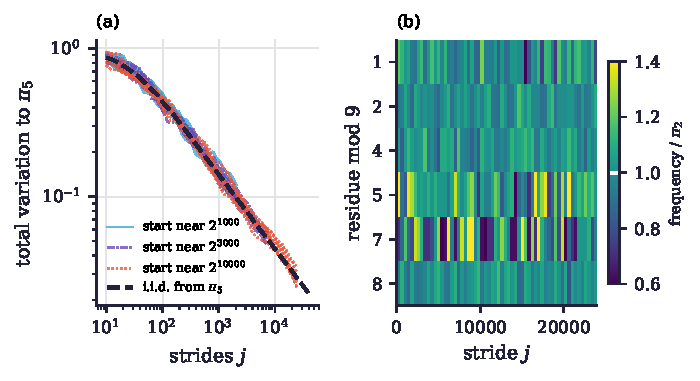
\includegraphics[width=\textwidth]{figures/ch9_orbits.pdf}
\caption{Equidistribution along single orbits. (a) Total variation distance
between the empirical distribution of $y_j\bmod3^5$ along an orbit and the
stationary law $\pi_5$, for $24$ orbits started near $2^{1000}$, $2^{3000}$ and
$2^{10000}$, against the mean distance for independent samples from $\pi_5$
(dashed). (b) Residue frequencies modulo $9$ along one orbit from near
$2^{10000}$, in windows of $400$ strides, relative to $\pi_2$.}
\label{fig:ch9:orbits}
\end{figure}

\section{Three routes and where they fail}\label{sec:ch9:routes}

We end by comparing three routes to the divergence half, each natural, each
developed somewhere in this book, and each failing.

\paragraph{Equidistribution.} If the iterates $y_j$ were equidistributed modulo $2^m$, for every $m$, along every divergent orbit, then $\liminf_N\bar k_N\ge2$ along it by \cref{prop:geom}, which \cref{cor:ch9:freq} forbids; there would be no divergent orbit, and \cref{conj:cesaro} would follow with room to spare.
No such statement can be asked of every orbit, since an orbit that reaches $1$ is eventually constant.
What is known concerns random starting values. Their first halving exponents are close in total variation to independent Geometric$(\tfrac12)$ draws~\cite[Proposition~1.9]{tao2022}, and the deep input of Tao\index{Tao, T.}'s theorem is a fine scale mixing estimate modulo powers of $3$~\cite[Proposition~1.14]{tao2022}.
The theorem establishes a form of equidistribution\index{equidistribution}, but on the $3$ adic side,
in logarithmic density over starting values, and with an exceptional set.
\Cref{lem:ch9:mixing} gives the finite analogue,
exact mixing\index{mixing} of the model chain. Every one of these statements is about an
ensemble or about a Markov chain built from one; the passage from an ensemble
to a single orbit is the step that is missing.

\paragraph{A Lyapunov certificate.} One would like a function $W$ and a constant
$\rho<1$ with $W(S(x))\le\rho W(x)$ for every odd $x\geq3$, which would give
geometric descent with no probabilistic content. \Cref{thm:nolyapunov} rules
this out for every $W$ increasing in $x$, since $S(x)>x$ on the whole class
$x\equiv3\pmod4$, and \cref{cor:ch4:multistride} rules out such $W$ at every fixed number
of strides, since ascents can be chained. A certificate\index{certificate} would have to depend on
the arithmetic of $x$. Certificates of that kind exist if the conjecture holds, for then $W(x)=2^{N(x)}$, where $N(x)$ is the number of strides from $x$ to $1$, satisfies $W(S(x))=\tfrac12W(x)$; but such a certificate, like the total stopping time\index{stopping time} it is built from, presupposes the conjecture. The functions that
do decrease, $\log x$ and $x^p$ for $0<p<1$, decrease in expectation
over a residue class, which is again an ensemble.

\paragraph{Uniform integrability.} Optional stopping for the
martingale\index{martingale} formed by the iterates of the model does not get started: stopped when it first drops to $1$ or below, the martingale is not uniformly integrable\index{uniform integrability} (\cref{prop:uimartingale}), and for the deterministic map the corresponding invariant function, the indicator of reaching $1$, exists trivially, while showing that it equals $1$ everywhere is the conjecture itself (\cref{rem:ch3:cert}). Above all, every martingale here lives on a
probability space of random parities. For a deterministic orbit there is no
filtration with respect to which $\log y_N-N\log\frac34$ is a martingale.

Two of the three failures have the same form: equidistribution and uniform integrability each replace a
statement about a specific trajectory by a statement about a measure, and in
each case the replacement is the step that cannot be justified. A pointwise certificate involves no measure and fails differently: no increasing $W$ works at any fixed number of strides, and the certificates that would work presuppose the answer. The heuristic
is not weak.
Its predictions match the data closely in the tests of this book and of the literature, the total stopping time slope to within about two percent and the variance of the stopping times to about ten percent (\cref{chap:stochastic}).
What is missing is a mechanism that transfers statistics from an ensemble to an
individual orbit, in the presence of a deterministic map that, as far as anyone
knows, has no special structure that would supply one. The Ces\`aro identity
makes the target precise: an orbit that reaches $1$ automatically has
$\bar k_N>\lt$, and an orbit that diverges automatically has
$\limsup\bar k_N\le\lt$. The divergence half of the Collatz conjecture\index{Collatz conjecture} is the
assertion that the second never happens, and the margin of $0.415$ between
the Geometric mean $2$ of the model and the threshold $\lt$ is, so far, a margin that no
argument has been able to transfer to a single orbit.

\section*{Notes}

The observation that a divergent orbit must contain a fraction of odd steps of
at least $1/\lt$ is elementary and has been made many times; it is the
divergence counterpart of the cycle inequality $3^m<2^k$ of \cref{chap:cycles}.
The Ces\`aro identity is the stride formula \eqref{eq:ch2:stride} summed along an orbit, and the pitfall of \cref{rem:ch9:circular} is an immediate consequence of it. The statement that almost every orbit falls below its starting value
is due to Terras\index{Terras, R.}~\cite{terras1976,terras1979} and Everett\index{Everett, C. J.}~\cite{everett1977}; the
exponent $\log3/\log4$ is due to Korec\index{Korec, I.}~\cite{korec1994}. The survey of
Lagarias\index{Lagarias, J. C.}~\cite{lagarias1985} and the volume~\cite{lagarias2010} contain much
more on the $2$ adic picture of \cref{rem:ch9:adic}.

Tao\index{Tao, T.}'s theorem appeared in~\cite{tao2022}; the paper is long but very clearly
written, and its introduction contains an excellent account of the
difficulties described in \cref{sec:ch9:tao}. The
Syracuse random variables and the fine scale mixing\index{mixing} estimate are defined and
proved there, and so are the identities behind the model chain of \cref{sec:ch9:spectral}: the loss of memory~\cite[eq.~(1.21)]{tao2022}, the one step recursion~\cite[Lemma~1.12]{tao2022} and the stationary law~\cite[Remark~1.13]{tao2022}. \Cref{lem:ch9:mixing} restates them in the form of a finite Markov chain. The counting bound
$\pi_1(x)\geq x^{0.84}$ is from Krasikov\index{Krasikov, I.} and Lagarias~\cite{krasikov2003}. The branching random
walk model for the tree of preimages is in Lagarias and Weiss\index{Weiss, A.}~\cite{lagarias1992}.

\begin{sloppypar}
All numerical results in this chapter were computed by the authors with the scripts \texttt{ch9\_spectral.py}, \texttt{ch9\_table.py}, \texttt{ch9\_figures.py}, \texttt{ch9\_numbers.py}, \texttt{ch9\_orbits.py} and \texttt{ch9\_orbits\_check.py} of the code appendix, and the scan of \cref{rem:ch9:circular} with \texttt{ch9\_cesaro\_scan.py}.
\end{sloppypar}

\section*{Exercises}

\begin{exercise}\label{ex:ch9:standard}
State and prove the analogue of \cref{prop:cesaro} for the standard map\index{standard map} $T_0$,
in terms of the number of odd steps among the first $n$ steps. Deduce the
second frequency statement of \cref{cor:ch9:freq} directly.
\end{exercise}

\begin{exercise}\label{ex:ch9:fivex}
For the $5x+1$ map with Syracuse form $y\mapsto(5y+1)/2^{\vt(5y+1)}$, derive
the Ces\`aro identity and show that an orbit that reaches $1$ must have
$\bar k_N>\log_25$. Under the Geometric law the mean exponent is still $2$.
What does this suggest about typical orbits of the $5x+1$ map?
\end{exercise}

\begin{exercise}\label{ex:ch9:mod9}
Compute the matrix $P_2$ of \eqref{eq:ch9:P} on the six units modulo $9$, check
that $P_2^{\,2}$ has identical columns, and verify that they equal
$\tfrac1{63}(8,16,11,4,2,22)$.
\end{exercise}

\begin{exercise}\label{ex:ch9:restricted}
Let $R$ be the operation that deletes from a column stochastic matrix on the
eighteen units modulo $27$ the rows and columns of the nine units with even
representatives in $[0,27)$, and renormalizes the remaining columns. Show that
the limiting nine state matrix of \cref{rem:ch9:oddreps} is $R(P_3)$, that
$R(P_3^{\,3})$ has rank one, and that $R(P_3)^3$ does not. Conclude that the
eigenvalues of the restricted matrix need not reflect the exact mixing\index{mixing} of
\cref{lem:ch9:mixing}.
\end{exercise}

\begin{exercise}\label{ex:ch9:entropy}
Let $q\in(\tfrac12,1)$. Show that the number of binary words of length $n$ with
at least $qn$ ones is $2^{nH(q)+o(n)}$. Using \cref{thm:terras}, deduce that the
proportion of residue classes modulo $2^n$ whose first $n$ accelerated steps
contain at least $n/\lt$ odd steps tends to zero exponentially, and compute
the rate.
\end{exercise}

\begin{exercise}\label{ex:ch9:tao}
Let $K_1,K_2,\ldots$ be independent Geometric$(\tfrac12)$. Compute the law of
$\sum_{m=1}^{3}3^{m-1}2^{-(K_1+\cdots+K_m)}\bmod27$ numerically, and compare it
with the stationary law of $P_3$. Then compute the fine scale discrepancy
$\sum_Y|\pi_3(Y)-\tfrac13\pi_2(Y\bmod9)|$.
\end{exercise}
